Предположим, что алгоритм двойного дерева имеет доступ к оракулу, который по полученному алгоритмом
эйлерову графу выбирает его оптимальный обход и оптимальную последовательность сокращений этого
обхода. Докажите, что даже в этом случае алгоритм двойного дерева для задачи коммивояжера с неравенством
треугольника~--- не $\alpha$-приближённый ни для какого $\alpha < 5 / 6$.

\answer{
    Пример в метрике кратчайших путей (число вершин во внешних лучах $n\to\infty$). На иллюстрации граф,
    удвоенное MST веса $12n + \bigO{1}$, оптимальное сокращение MST веса $10n + \bigO{1}$, оптимальный
    обход графа веса $6n + \bigO{1}$.

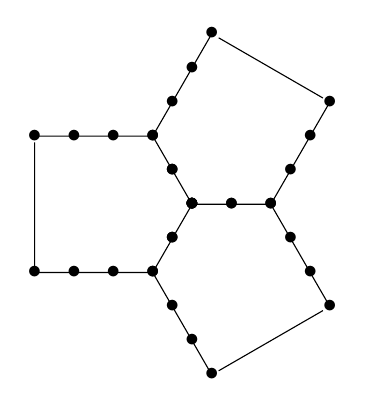
\begin{tikzpicture}[baseline=(base),inner sep=0pt,outer sep=0pt]
\draw (0,0) coordinate(base)
(0,0) node{$\bullet$} -- ++(0:0.5) node{$\bullet$} -- ++(0:0.5) node{$\bullet$} 
-- ++(-60:0.5) node{$\bullet$} -- ++(-60:0.5) node{$\bullet$} -- ++(-60:0.5) node(a){$\bullet$} 
(0,0) node{$\bullet$} -- ++(0:0.5) node{$\bullet$} -- ++(0:0.5) node{$\bullet$} 
-- ++(60:0.5) node{$\bullet$} -- ++(60:0.5) node{$\bullet$} -- ++(60:0.5) node(b){$\bullet$} 
(0,0) node{$\bullet$} -- ++(120:0.5) node{$\bullet$} -- ++(120:0.5) node{$\bullet$} 
-- ++(60:0.5) node{$\bullet$} -- ++(60:0.5) node{$\bullet$} -- ++(60:0.5) node(c){$\bullet$} 
(0,0) node{$\bullet$} -- ++(120:0.5) node{$\bullet$} -- ++(120:0.5) node{$\bullet$} 
-- ++(180:0.5) node{$\bullet$} -- ++(180:0.5) node{$\bullet$} -- ++(180:0.5) node(d){$\bullet$} 
(0,0) node{$\bullet$} -- ++(240:0.5) node{$\bullet$} -- ++(240:0.5) node{$\bullet$} 
-- ++(180:0.5) node{$\bullet$} -- ++(180:0.5) node{$\bullet$} -- ++(180:0.5) node(e){$\bullet$} 
(0,0) node{$\bullet$} -- ++(240:0.5) node{$\bullet$} -- ++(240:0.5) node{$\bullet$} 
-- ++(300:0.5) node{$\bullet$} -- ++(300:0.5) node{$\bullet$} -- ++(300:0.5) node(f){$\bullet$} 
(b) -- (c) (d) -- (e) (f) -- (a);
\end{tikzpicture}
\qquad
%
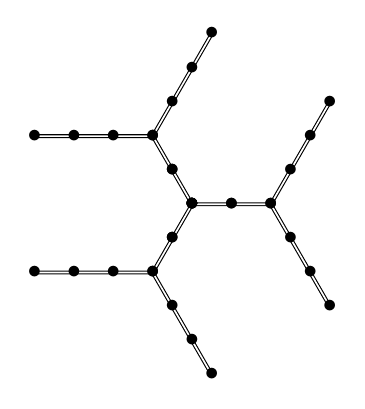
\begin{tikzpicture}[baseline=(base),inner sep=0pt,outer sep=0pt]
\draw[double] (0,0) coordinate(base)
(0,0) node{$\bullet$} -- ++(0:0.5) node{$\bullet$} -- ++(0:0.5) node{$\bullet$} 
-- ++(-60:0.5) node{$\bullet$} -- ++(-60:0.5) node{$\bullet$} -- ++(-60:0.5) node(a){$\bullet$} 
(0,0) node{$\bullet$} -- ++(0:0.5) node{$\bullet$} -- ++(0:0.5) node{$\bullet$} 
-- ++(60:0.5) node{$\bullet$} -- ++(60:0.5) node{$\bullet$} -- ++(60:0.5) node(b){$\bullet$} 
(0,0) node{$\bullet$} -- ++(120:0.5) node{$\bullet$} -- ++(120:0.5) node{$\bullet$} 
-- ++(60:0.5) node{$\bullet$} -- ++(60:0.5) node{$\bullet$} -- ++(60:0.5) node(c){$\bullet$} 
(0,0) node{$\bullet$} -- ++(120:0.5) node{$\bullet$} -- ++(120:0.5) node{$\bullet$} 
-- ++(180:0.5) node{$\bullet$} -- ++(180:0.5) node{$\bullet$} -- ++(180:0.5) node(d){$\bullet$} 
(0,0) node{$\bullet$} -- ++(240:0.5) node{$\bullet$} -- ++(240:0.5) node{$\bullet$} 
-- ++(180:0.5) node{$\bullet$} -- ++(180:0.5) node{$\bullet$} -- ++(180:0.5) node(e){$\bullet$} 
(0,0) node{$\bullet$} -- ++(240:0.5) node{$\bullet$} -- ++(240:0.5) node{$\bullet$} 
-- ++(300:0.5) node{$\bullet$} -- ++(300:0.5) node{$\bullet$} -- ++(300:0.5) node(f){$\bullet$};
\end{tikzpicture}
\qquad
%
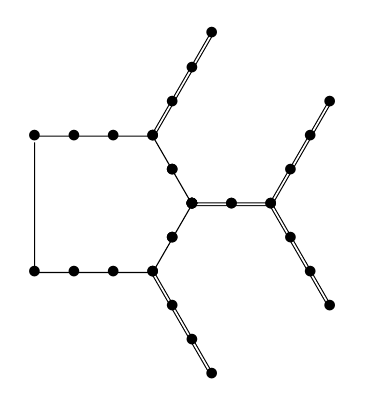
\begin{tikzpicture}[baseline=(base),inner sep=0pt,outer sep=0pt]
\draw[double] (0,0) coordinate(base)
(0,0) node{$\bullet$} -- ++(0:0.5) node{$\bullet$} -- ++(0:0.5) node{$\bullet$} 
-- ++(-60:0.5) node{$\bullet$} -- ++(-60:0.5) node{$\bullet$} -- ++(-60:0.5) node(a){$\bullet$} 
(0,0) node{$\bullet$} -- ++(0:0.5) node{$\bullet$} -- ++(0:0.5) node{$\bullet$} 
-- ++(60:0.5) node{$\bullet$} -- ++(60:0.5) node{$\bullet$} -- ++(60:0.5) node(b){$\bullet$} 
(0,0) node{$\bullet$} ++(120:0.5) node{$\bullet$} ++(120:0.5) node{$\bullet$} 
-- ++(60:0.5) node{$\bullet$} -- ++(60:0.5) node{$\bullet$} -- ++(60:0.5) node(c){$\bullet$} 
(0,0) node{$\bullet$} ++(240:0.5) node{$\bullet$} ++(240:0.5) node{$\bullet$} 
-- ++(300:0.5) node{$\bullet$} -- ++(300:0.5) node{$\bullet$} -- ++(300:0.5) node(f){$\bullet$};
\draw (0,0)
(0,0) node{$\bullet$} -- ++(120:0.5) node{$\bullet$} -- ++(120:0.5) node{$\bullet$} 
-- ++(180:0.5) node{$\bullet$} -- ++(180:0.5) node{$\bullet$} -- ++(180:0.5) node(d){$\bullet$}
(0,0) node{$\bullet$} -- ++(240:0.5) node{$\bullet$} -- ++(240:0.5) node{$\bullet$} 
-- ++(180:0.5) node{$\bullet$} -- ++(180:0.5) node{$\bullet$} -- ++(180:0.5) node(e){$\bullet$} 
(d) -- (e);
\end{tikzpicture}

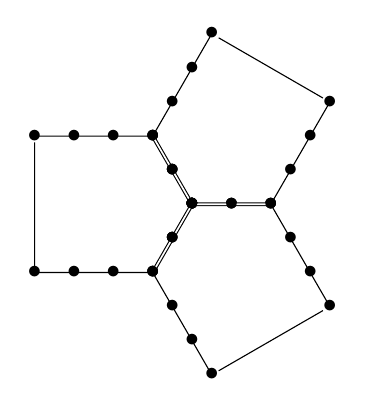
\begin{tikzpicture}[baseline=(base),inner sep=0pt,outer sep=0pt]
\draw (0,0) coordinate(base)
(0,0) node{$\bullet$} ++(0:0.5) node{$\bullet$} ++(0:0.5) node{$\bullet$} 
-- ++(-60:0.5) node{$\bullet$} -- ++(-60:0.5) node{$\bullet$} -- ++(-60:0.5) node(a){$\bullet$} 
(0,0) node{$\bullet$} ++(0:0.5) node{$\bullet$} ++(0:0.5) node{$\bullet$} 
-- ++(60:0.5) node{$\bullet$} -- ++(60:0.5) node{$\bullet$} -- ++(60:0.5) node(b){$\bullet$} 
(0,0) node{$\bullet$} ++(120:0.5) node{$\bullet$} ++(120:0.5) node{$\bullet$} 
-- ++(60:0.5) node{$\bullet$} -- ++(60:0.5) node{$\bullet$} -- ++(60:0.5) node(c){$\bullet$} 
(0,0) node{$\bullet$} ++(120:0.5) node{$\bullet$} ++(120:0.5) node{$\bullet$} 
-- ++(180:0.5) node{$\bullet$} -- ++(180:0.5) node{$\bullet$} -- ++(180:0.5) node(d){$\bullet$} 
(0,0) node{$\bullet$} ++(240:0.5) node{$\bullet$} ++(240:0.5) node{$\bullet$} 
-- ++(180:0.5) node{$\bullet$} -- ++(180:0.5) node{$\bullet$} -- ++(180:0.5) node(e){$\bullet$} 
(0,0) node{$\bullet$} ++(240:0.5) node{$\bullet$} ++(240:0.5) node{$\bullet$} 
-- ++(300:0.5) node{$\bullet$} -- ++(300:0.5) node{$\bullet$} -- ++(300:0.5) node(f){$\bullet$} 
(b) -- (c) (d) -- (e) (f) -- (a);
\draw[double]
(0,0) node{$\bullet$} -- ++(0:0.5) node{$\bullet$} -- ++(0:0.5) node{$\bullet$} 
(0,0) node{$\bullet$} -- ++(120:0.5) node{$\bullet$} -- ++(120:0.5) node{$\bullet$} 
(0,0) node{$\bullet$} -- ++(240:0.5) node{$\bullet$} -- ++(240:0.5) node{$\bullet$};
\end{tikzpicture}

В евклидовой метрике аналогичный пример дает нижнюю оценку 
$(8 + \sqrt{3})/6 \approx 1.622 < 5/3$.
}